\documentclass[a4paper]{article}
\usepackage{amsfonts}
\usepackage{amsmath}
\usepackage{amssymb}
\usepackage{graphicx}	

\begin{document}
  
\noindent \large Auteur: Niels Hertoghs \\
\noindent \large Studierichting: Informatica\\
\noindent \large Oefeningenreeks 3G nr 7.5 \\

\medskip

\normalsize


$f(x) = (x-1)(x-2)(x-3) = x^3-6x^2+11x-6$ \\

$\operatorname{dom}f: x \in \mathbb{R}$ \\

$\Rightarrow $nulpunten: $x = 1,x = 2, x = 3$\\

Assymptoten: \\

Geen VA want $\operatorname{dom} f(x)=\mathbb{R}$\\

HA:$\lim\limits_{x\rightarrow \infty} f(x) = \infty \Rightarrow $geen HA\\

SA:$\lim\limits_{x\rightarrow \infty} \dfrac{f(x)}{x}= \infty \Rightarrow $geen SA\\

$f'(x) = 3x^2-12x+11$  \\

$\Rightarrow $nulpunten: $3x^2-12x+11 = 0 \Rightarrow D = 12$\\

$x_1 = 2+\dfrac{\sqrt{3}}{3}$\\

$x_2 = 2-\dfrac{\sqrt{3}}{3}$\\

$f''(x) = 6x-12$ \\

$\Rightarrow $nulpunten: $6x-12 = 0 \Rightarrow x = 2$\\

\begin{tabular}{c|ccccccccccc}
$x$				&		& $1$ &  & $2-\dfrac{\sqrt{3}}{3}$ &  & $2$ &  & $2+\dfrac{\sqrt{3}}{3}$ &  & $3$ & \\ \hline
$f(x)$		& $-$ & $0$ & $+$ & $+$ & $+$ & $0$ & $-$ & $-$ & $-$ & $0$ & $+$ \\
$f'(x)$		& $+$ & $+$ & $+$ & $0$ & $-$ & $-$ & $-$ & $0$ & $+$ & $+$ & $+$ \\
$f''(x)$	& $-$ & $-$ & $-$ & $-$ & $-$ & $0$ & $+$ & $+$ & $+$ & $+$ & $+$ \\ \hline
$f(x)$		& $\nearrow$ & $\nearrow$ & $\nearrow$ & $M\left(\dfrac{2\sqrt{3}}{9}\right)$ & $\searrow$ & $\searrow$ &$\searrow$ & $m\left(\dfrac{-2\sqrt{3}}{9}\right)$ & $\nearrow$ & $\nearrow$ & $\nearrow$ \\
					& $\frown$ & $\frown$ & $\frown$ & $\frown$ & $\frown$ & $0$ & $\smile$ & $\smile$ & $\smile$ & $\smile$ & $\smile$ \\
\end{tabular}  \\

Tekening: \\

\begin{figure}[h]
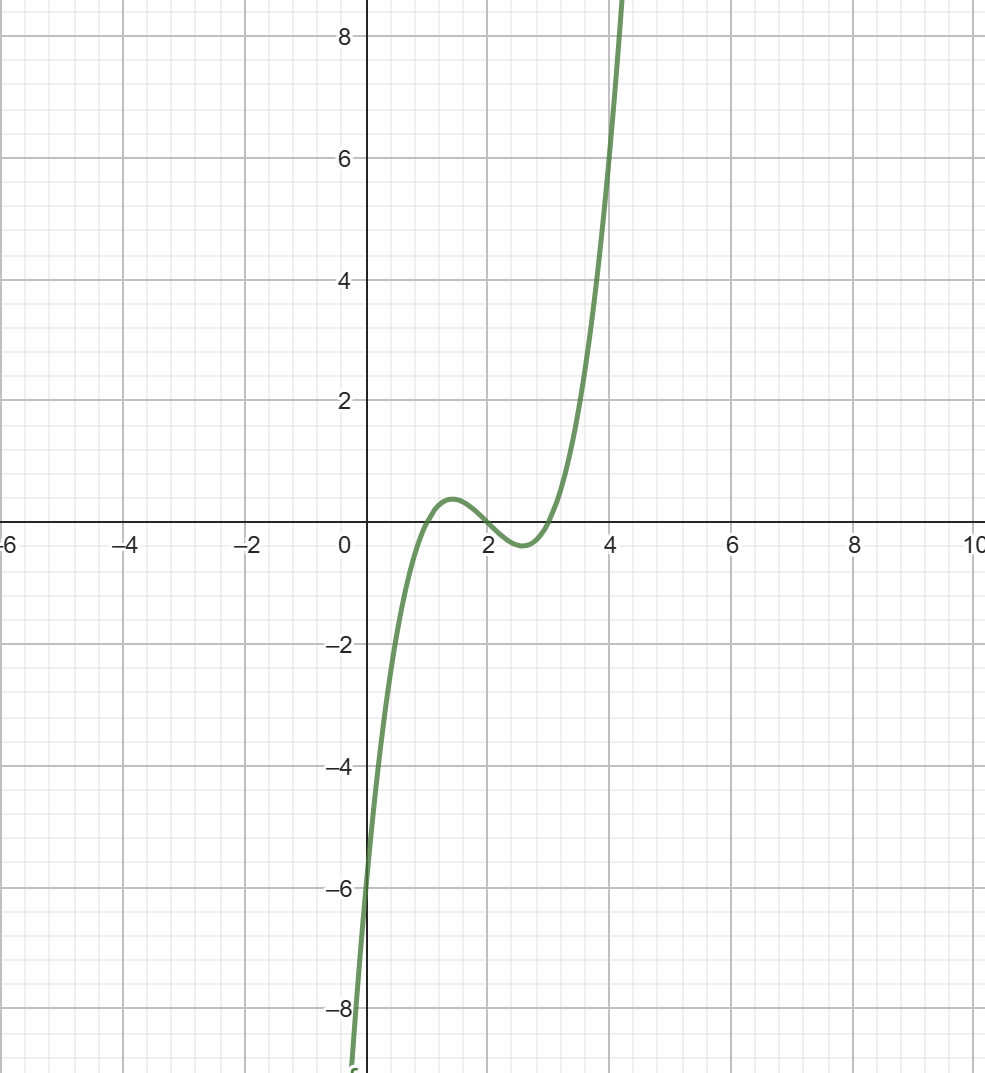
\includegraphics[width=\linewidth]{3G-7.5-niels.hertoghs.INF.png}\\
\end{figure} 


\begin{thebibliography}{999}
%\bibitem{a} Referentie
\end{thebibliography}
\end{document} 
^